\documentclass{report}
\usepackage{titlesec}
\title{Instructions for Creating an Analysis Environment with Anaconda}
\author{Liam O'Suilleabhain}
\date{\today}

\usepackage{graphicx}
\usepackage{caption}
\usepackage{amsmath}
\usepackage{algorithm}
\usepackage{hyperref} 

\usepackage[noend]{algorithmic}
\titleformat{\chapter}[block]
  {\normalfont\huge\bfseries}{\thechapter.}{1em}{\Huge}
\titlespacing*{\chapter}{0pt}{-19pt}{0pt}


\usepackage{Sweave}
\begin{document}

\maketitle

\chapter*{Development Directory}

Here, we are going to define the root directory of our analysis environment.

\begin{figure}[H]
\centering
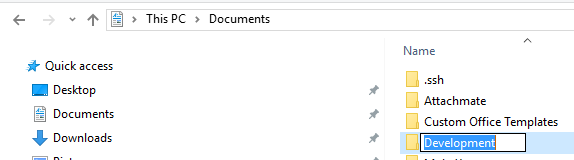
\includegraphics{./images/Development.PNG}
\caption{The Root Directory of our Analysis Environment is set to Development}
\end{figure}


\chapter*{Installation of Miniconda}

\bigskip
This section describes steps for installing the Anaconda package manager (Miniconda) for 64-bit Windows 10 laptops and Desktops. \\

\hypertarget{download-miniconda-3-for-64-bit-windows}{%
\section*{\texorpdfstring{\href{https://conda.io/miniconda.html}{Download} 
Miniconda for 64-bit Windows}{Download Miniconda}}\label{download-miniconda-3-for-64-bit-windows}}

\subsection*{Open the Executable}

\begin{figure}[h!]
\centering
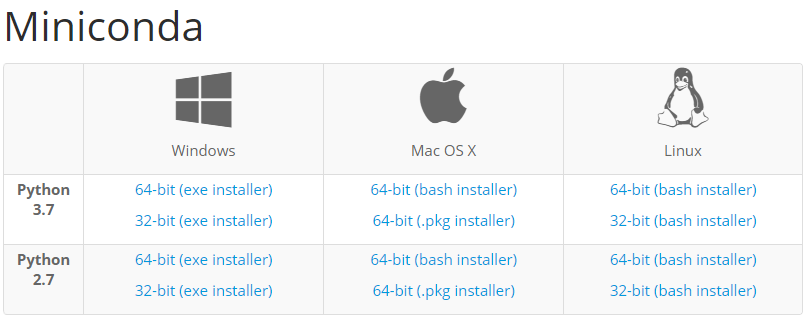
\includegraphics{./images/miniconda3.PNG}
\caption{Click on the python3.7 64-bit Windows (exe-installer).}
\end{figure}

\begin{figure}[H]
\centering
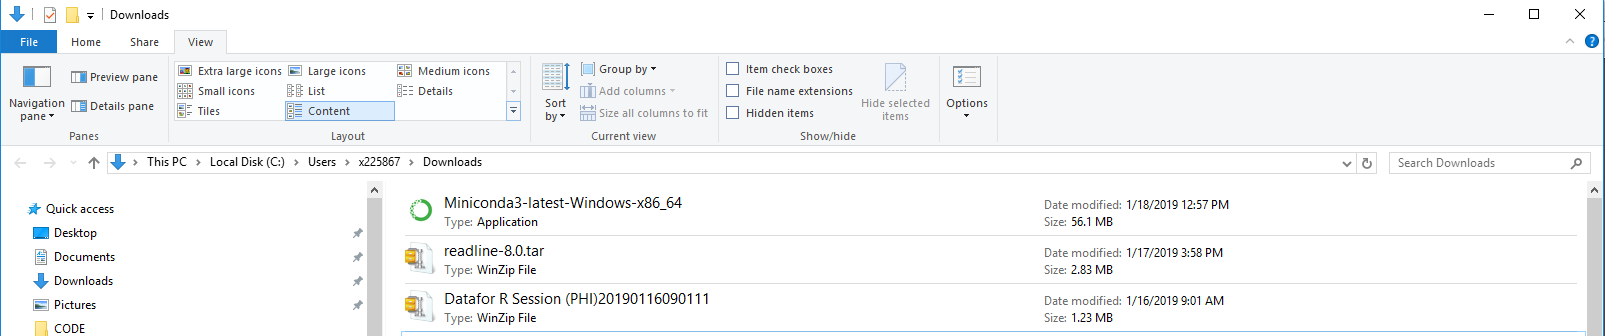
\includegraphics[width=1.2\textwidth]{./images/download.PNG}
\caption{Double click on the file downloaded}
\end{figure}


\section*{Installation Process}

\begin{figure}[H]
\centering
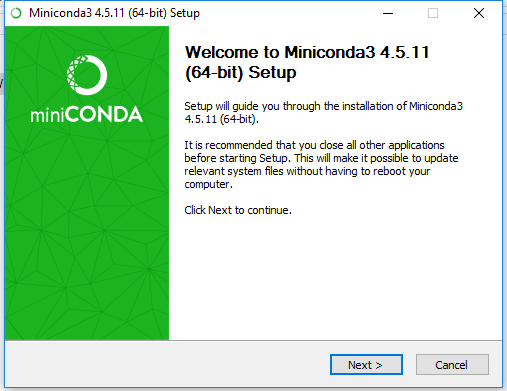
\includegraphics{./images/Welcome.PNG}
\caption{Baby Steps}
\end{figure}

\begin{figure}[H]
\centering
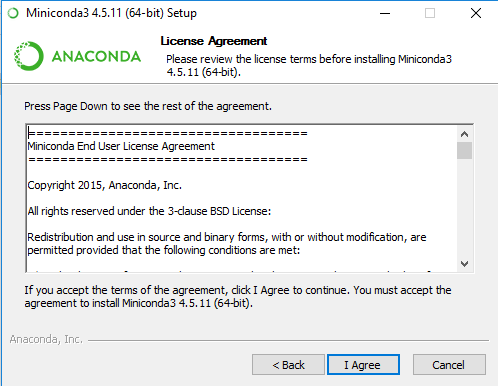
\includegraphics{./images/Liscence.PNG}
\caption{BSD licenses are a family of permissive free software licenses, imposing minimal restrictions on the use and redistribution of covered software.}
\end{figure}

\begin{figure}[H]
\centering
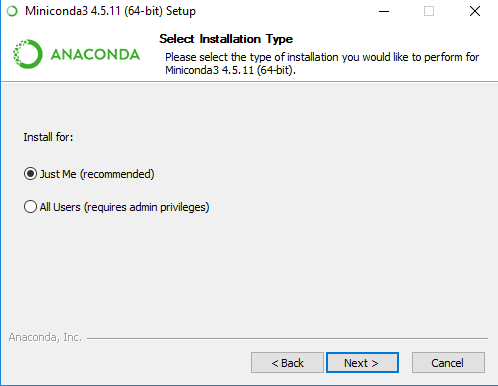
\includegraphics{./images/Just_Me.PNG}
\caption{Select the first option (Just Me)}
\end{figure}

\subsection*{Select Installation Directory}

\begin{figure}[H]
\centering
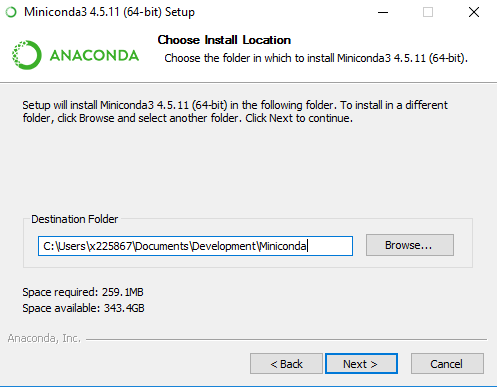
\includegraphics{./images/Installation_Directory.PNG}
\caption{You must install to a new folder in the Development directory}
\end{figure}

\subsection*{Advanced Options}
\begin{figure}[H]
\centering
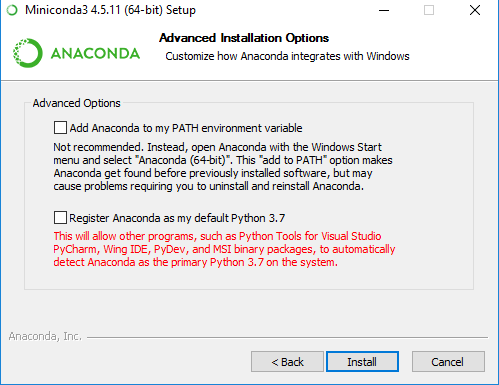
\includegraphics{./images/Isolated_Installation.PNG}
\caption{isolate\_install}
\end{figure}

\begin{center}
\textbf{N.B. Unselect "Register Anaconda in my default Python 3.7".} You will not be able to select this unless you have administrative priveleges.
\end{center}


\begin{figure}[H]
\centering
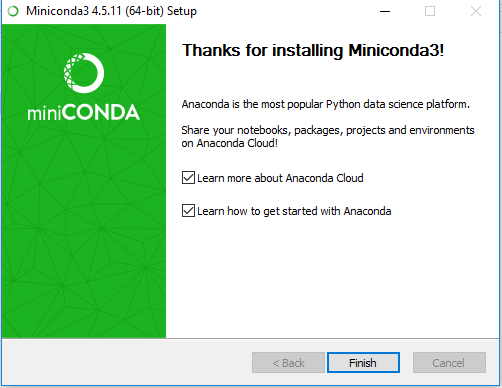
\includegraphics[width=0.75\textwidth]{./images/Finish.PNG}
\caption{Finish}
\end{figure}

 % Add a bibliography block to the postdoc
    
\chapter*{Installation of Jupyter}
\bigskip
This section involves installation and configuration of jupyter. 

\section*{Anaconda Prompt}
\begin{figure}[H]
\centering
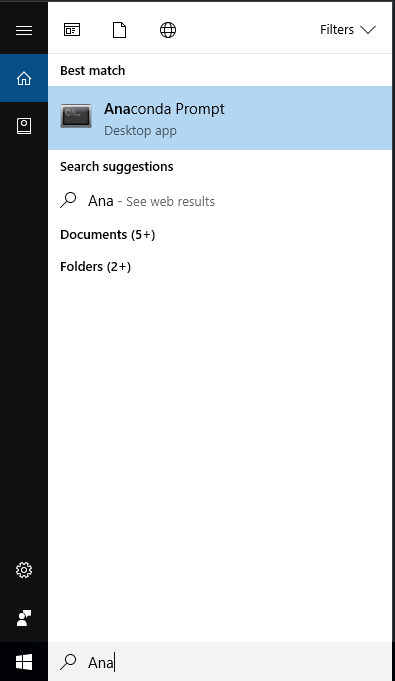
\includegraphics[width=0.4\textwidth]{./images/Prompt.PNG}
\caption{Press Windows hotkey and open Anaconda}
\end{figure}

\begin{Large}\begin{center}\textbf{Submit the following command at the prompt}\end{center}\end{Large}
\begin{center}
conda install jupyter
\end{center}

\begin{Large}\begin{center}\textbf{Create a Jupyter Notebook Configuration File}\end{center}\end{Large}

\begin{figure}[H]
\centering
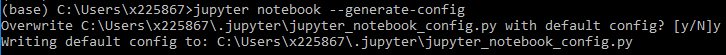
\includegraphics{./images/generate_configuration_file.PNG}
\caption{``jupyter notebook --generate-config'' generates a configuration file}
\end{figure}

\subsection*{Find .jupyter in File Explorer}

\begin{figure}[H]
\centering
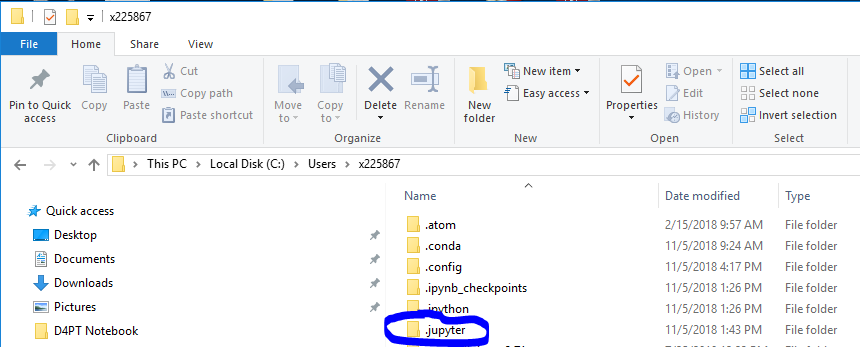
\includegraphics{./images/jupyter_configuration_file.PNG}
\caption{Open .jupyter folder (eg C:/Users/x225867/.jupyter)}
\end{figure}

NB Because the folder ``.jupyter'' has a dot preceding its name, it is a ``hidden file''. To view hidden files modify your view settings in file explorer.


\subsection*{Edit Configuration File}

The goal is to modify the directory where the notebook opens. 

\begin{figure}[H]
\centering
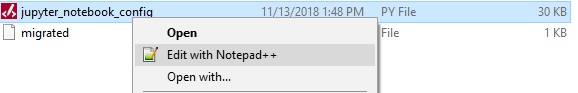
\includegraphics{./images/jupyter_configuration_edit.PNG}
\caption{Edit jupyter\_notebook\_config with notepad++}
\end{figure}

\textbf{Set notebook\_dir to Development directory (line 262 in my file)}\\
c.NotebookApp.notebook\_dir='C:/Users/x225867/Documents/Development/'\\

In order for jupyter to see the new directory, We need to remove the ``\#'' symbol before c.NotebookApp.notebook\_dir.

\begin{figure}[H]
\centering
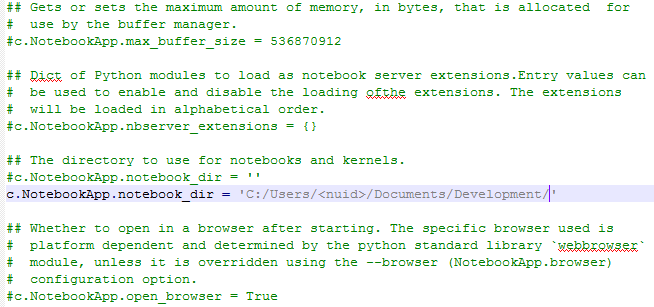
\includegraphics{./images/notebook_dir.PNG}
\caption{Configure Jupyter to open in your analysis environment.}
\end{figure}

\section*{\texorpdfstring{
\href{https://guides.github.com/features/mastering-markdown/}{Master
Markdown}}{Step N. Master Markdown}}

\chapter*{R, Rstudio and IRkernel}

This section brings our environment together; Rstudio is a useful IDE for working with R, and Jupyter allows us to communicate reproducible results in Python or R.

\section*{Start Anaconda Prompt}

\begin{figure}[H]
\centering
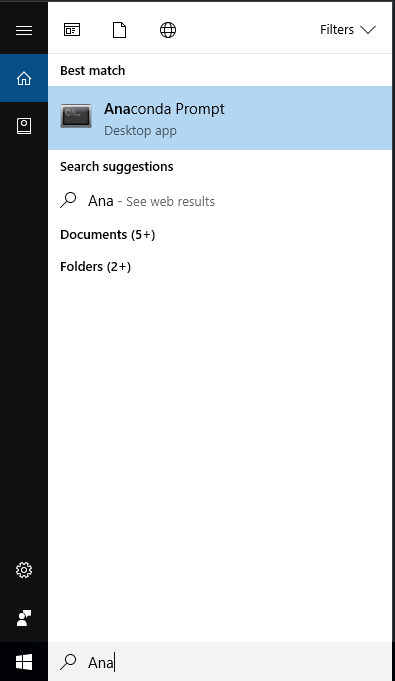
\includegraphics[width=0.5\textwidth]{./images/Prompt.PNG}
\caption{Start Anaconda Prompt}
\end{figure}

\section*{Install Base R}

\begin{figure}[H]
\centering
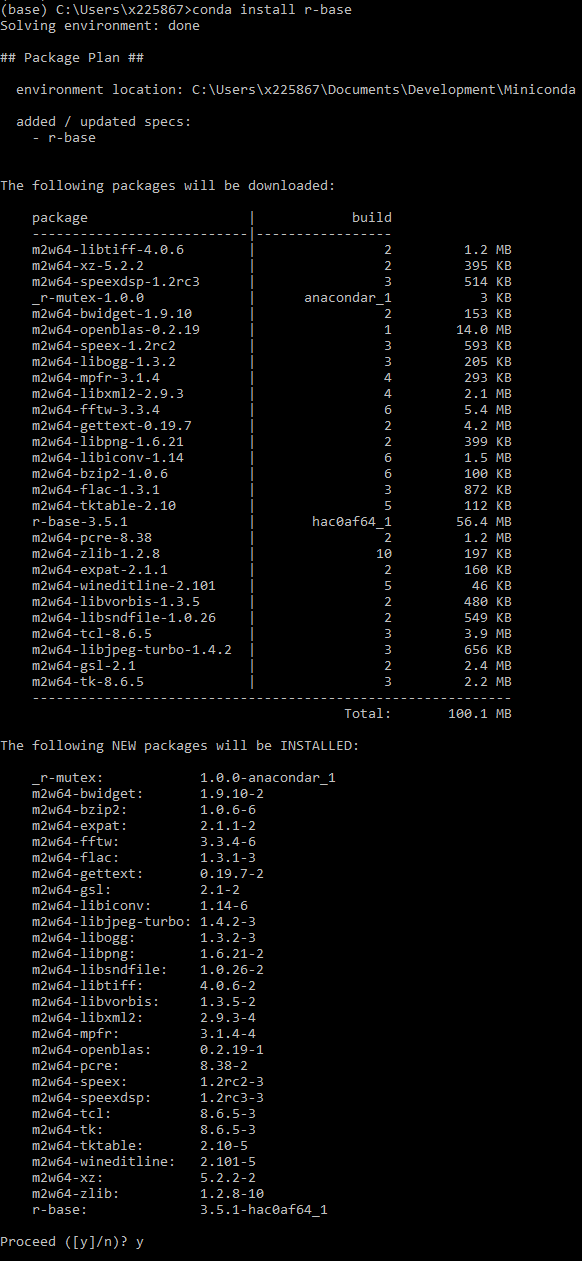
\includegraphics[width=0.65\textwidth]{./images/r_install.PNG}
\caption{conda install r-base}
\end{figure}

\section*{Install RStudio}

A ton of packages get installed, so expect a wait.

\begin{figure}[H]
\centering
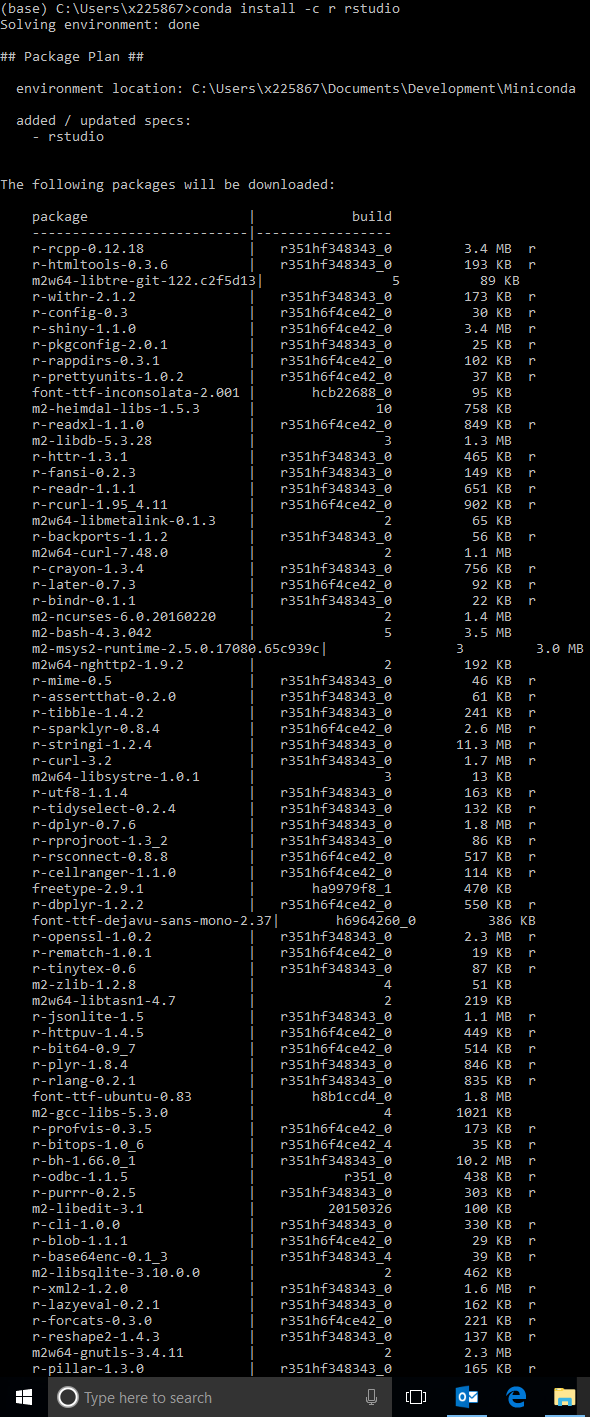
\includegraphics[width=0.55\textwidth]{./images/rstudio_install.PNG}
\caption{conda install -c r rstudio}
\end{figure}

\section*{Install IRkernel}

\begin{figure}[H]
\centering
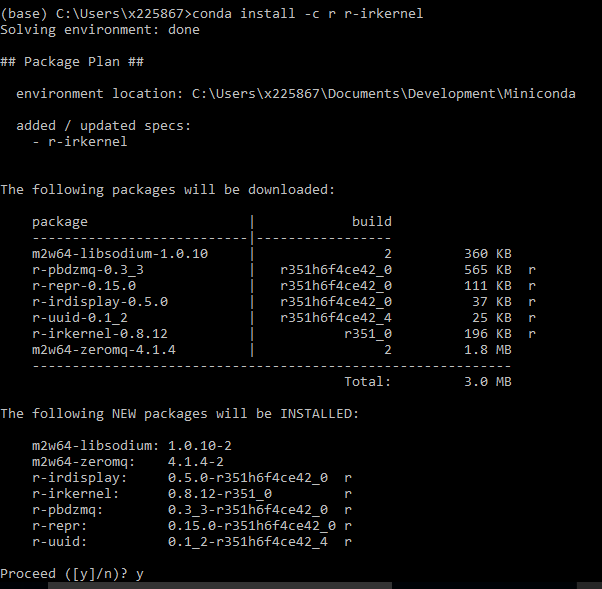
\includegraphics{./images/irkernel_install.PNG}
\caption{conda install -c r r-irkernel}
\end{figure}

\end{document}
